\lab{Complexity and Sparse Matrices}{Complexity and Sparse Matrices}

\objective{Introduce the temporal and spatial complexity and explore SciPy's methods for working with sparse matrices.}
\label{lab:complexity}

\section*{Complexity} 
Two major constraints on computing are time and available memory (or `space').
The \emph{temporal complexity} and \emph{spatial complexity} of an algorithm measure how much of these resources the algorithm requires. 
This lab intoduces complexity using examples and intuition; for a rigorous introduction, see Volume 2 of the textbook.

\subsection*{Temporal Complexity}
One of the most important questions in scientific computing is ``How long will a computer take to execute this algorithm?"
For example, suppose an algorithm operating on a 1-D array of length $n$ requires $f(n)$ calculations, where

\begin{equation*}
f(n) = \frac{3n^3}{2} + 75n^2 + 250n + 30.
\end{equation*}

As $n$ increases, the growth of $f(n)$ is dominated by the $n^3$ term.
This gives us information about how the runtime of our algorithm increases when we increase input size. 
If we double the size of the input $n$, we would expect the algorithm to need about $2^3=8$ times as many steps, which would make it run about 8 times as long.

The function $f(n)$ above is called the \emph{temporal complexity} of the algorithm. 
In general, $n$ is a positive integer that somehow describes the size of the inputs to your algorithm. 
For example, perhaps your algorithm accepts $n \times n$ arrays, or perhaps it accepts 1-D arrays of length $n$. 
The temporal complexity of your algorithm is a function that accepts an input size $n$ and returns the number of steps the algorithm needs to execute on that input. 
As such, temporal complexity is a precise way to describe how the execution time of your algorithm increases as the size of your input increases.

Often, we do not care about the exact definition of $f(n)$ so much as its behavior when $n$ gets large. 
This leads to the notion of an \emph{asymptotic upper bound}. 
An asymptotic upper bound is another function $g(n)$ such that, eventually, $f(n)$ is less than some constant multiple of $g(n)$. 
In the above example, $n^3$ is an asymptotic upper bound for $f(n)$ (see Figure \ref{fig:asymp_upper_bound}). 
If $g(n)$ is an asymptotic upper bound for $f(n)$, we say $f(n)$ is $O(g(n))$. 
So in the example above, $f(n)$ is $O(n^3)$ (spoken ``Big O of n cubed'' or ``order of n cubed").

\begin{figure}
\centering
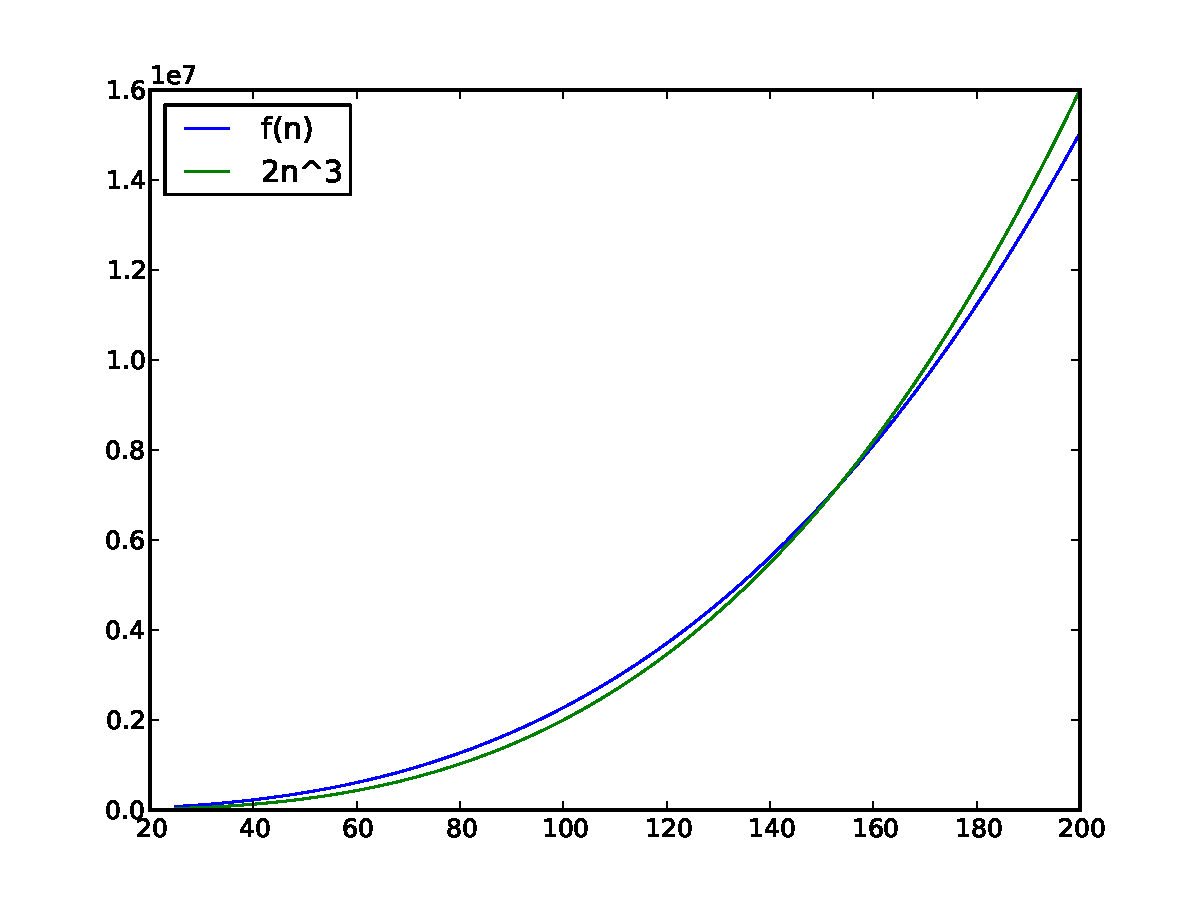
\includegraphics[width=\textwidth]{asymp_upper_bound.pdf}
\caption{When $n$ is bigger than 160, $f(n)$ is less than $2n^3$. This means that $n^3$ is an asymptotic upper bound for $f(n)$, so we say $f(n)$ is $O(n^3)$.}
\label{fig:asymp_upper_bound}
\end{figure}

For example, adding two $n \times n$ matrices is $O(n^2)$. 
This is because it takes 1 step to add each pair of elements in two $n \times n$ arrays, and there are $n^2$ such pairs.
By comparison, calculating the inverse of a $n \times n$ matrix using Gaussian row reduction is $O(n^3)$. 
(More efficient algorithms for matrix inversion exist as well.)

\begin{comment}
How do we determine the temporal complexity of a piece of code?
Calculating the exact temporal complexity of an algorithm is fairly difficult.
However, there are ways to heuristically evaluate the asymptotic behavior of an algorithm's temporal complexity. 
For example, consider the following code.

\begin{lstlisting}
s = 0
for i in xrange(n):
    s = s + i
\end{lstlisting}

The code above is $O(n)$ because it takes approximately $n$ steps to complete. 
For-loops are a good indicator of the complexity.  
A double for-loop suggests $O(n^2)$ or worse.  

You can also approximate the temporal complexity of a function by timing how long it takes to run on inputs of various sizes. 
This is especially useful if your temporal complexity is some polynomial. 
In this case, the ratios of the run times will give you clues about the temporal complexity of the algorithm. 
For example, if an algorithm is $O(n^3)$, then doubling the size of the input should make the algorithm take $(2n)^3/n^3=8$ times as long.
\begin{comment}
\begin{problem}
Time the runtime of the following code for \li{n = 1000, 2000, 4000, 8000}.

\lstinputlisting[style=fromfile]{test.py}

Now write a function that takes no arguments and does the following: 
\begin{enumerate}
\item Plots the four runtimes (use \li{[1000, 2000, 4000, 8000]} or an equivalent array object as your domain).
The plot should look like Figure \ref{prob1} if using the \li{plt.scatter} command. 
\item Returns the average ratio between successive runtimes (one such ratio would be the runtime for $n = 2000$ divided by the runtime for $n = 1000$).
\end{enumerate}
\begin{figure}
\centering
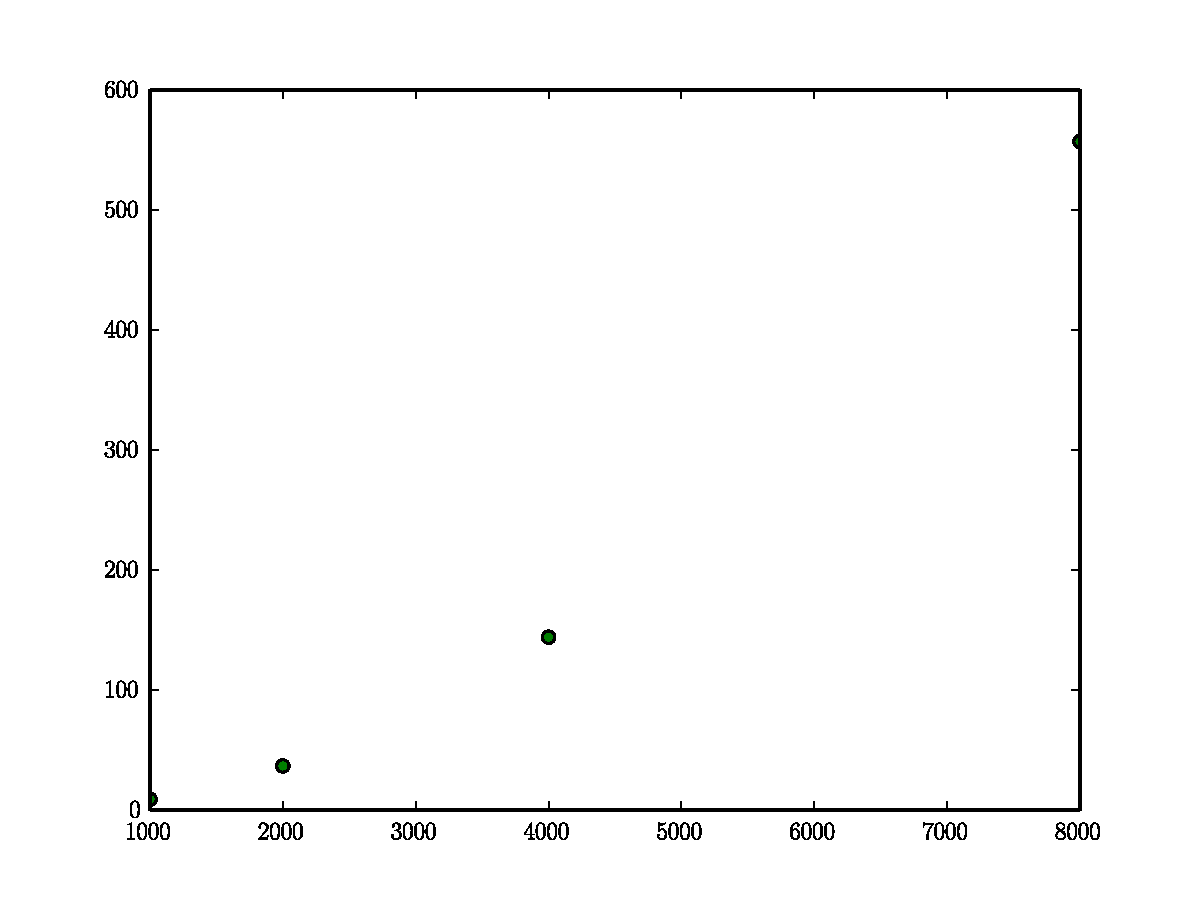
\includegraphics[width=\textwidth]{prob1.pdf}
\caption{The plot of problem 1}
\label{prob1}
\end{figure}
\end{problem}


\begin{problem}\label{complexity_ratios}
Fill in the following table. Here, $f(n)$ is the temporal complexity of an algorithm. The quantity $f(2n)/f(n)$ tells you how much longer each algorithm will take to run when you double the size of the input.

\begin{center}
\begin{tabular}{| l |p{15mm}|p{15mm}|p{15mm}|p{15mm}|p{15mm}|}\hline
$f(n)$ & $n$ & $n^2$ & $n^3$ & $n^4$  \\ \hline
$f(2n)/f(n)$&  & & &  \\
\hline
\end{tabular}
\end{center}

\end{problem}

\begin{problem}\label{complexity_timeit}
Determine the temporal complexity of each of the following functions. 
\begin{enumerate}
\item 
\begin{lstlisting}
def function1(n):
    t = 0
    for i in xrange(n):
        t += sum(xrange(i))
\end{lstlisting}

\item
\begin{lstlisting}
def function2(n):
    sum(xrange(1000*n))
\end{lstlisting}
\end{enumerate}

Do this as follows:
\begin{enumerate}
\renewcommand{\theenumi}{\alph{enumi}}
\item Time how long the function takes to run on an input of size $n$ for $n=1000, 2000, 4000$, and $8000$.
\item Compute the averages of the ratios between successive runtimes from part (1).
\item Use Problem \ref{prob:complexity_ratios} to determine the temporal complexity.
\end{enumerate}
\end{problem}

\begin{problem}
Create a plot depicting the complexities you found in Problem \ref{prob:complexity_timeit} by following these steps. 
\begin{enumerate}
\item For each function, plot a line using $n=1000, 2000, 4000$, and $8000$ for $x$-values and your runtimes for $y$-values. When you call the function \li{plt.plot()}, specify a value for the keyword parameter \li{label} so you can reference each line later. For example, the call \li{plt.plot( x, y, label="Function 1")} attaches the label "Function 1" to this line.
\item After plotting all your lines, call \li{plt.legend()} to draw a legend on your graph. Use the keyword argument \li{loc} to specify the location of the legend. Some possible values are \li{'upper left'} and \li{'right'}. See the documentation for more options.
\end{enumerate}
Your graph should look something like this.

[TODO: put a figure here]
\end{problem}
\end{comment}


\subsection*{Spatial Complexity}
Analogous to temporal complexity, the spatial complexity of an algorithm is a function that describes how the algorithm's memory use increases as input sizes to the algorithm increase. For example, if your algorithm needs to store an $n \times n$ matrix, its memory use will increase at least as fast as $n^2$. Spatial complexity is important because  the spatial complexity of an algorithm can affect its speed in several ways. The most important way is that when the memory usage exceeds the amount of available RAM, the machine must use either the hard disk or some other slower method of storage.

This vocabulary allows us to discuss the question at the start of this lab: ``How long will a computer take to execute this algorithm?" The amount of time a computer takes to execute an algorithm depends both on the algorithm's temporal complexity and on its spatial complexity. 

\subsection*{Timing Functions}
We can empirically investigate a function's temporal and spatial complexity by timing how long it takes to run.
In IPython\footnote{If you aren't using IPython, you will need
to use the timeit function documented here: \url{https://docs.python.org/2/library/timeit.html}.}, you can time a line of code by prefacing it with the command \li{\%timeit}.
As an example, we time how long it takes to add the numbers from 1 to 1000.
\begin{lstlisting}
>>> \%timeit sum(xrange(1000))
100000 loops, best of 3: 12.2 us per loop
\end{lstlisting}
This output means that the computer ran our line 100,000 times and averaged the runtimes.
The computer repeated this experiment 3 times, and the best average was 12.2 microseconds.

\begin{problem}\label{prob:complexity_problem}
In this problem you will analyze the complexity of the following functions:

\begin{lstlisting}
# Run through a single for loop.
def func1(n):
    n = 500*n
    sum(xrange(n))
# Run through a double for loop.
def func2(n):
    n = 3*n
    t = 0
    for i in xrange(n):
        for j in xrange(i):
            t += j
# Square a matrix.
def func3(n):
    n = int(1.2*n)
    A = np.random.rand(n, n)
    np.power(A, 2)
# Invert a matrix.
from scipy import linalg as la
def func4(n):
    A = np.random.rand(n, n)
    la.inv(A)
# Find the determinant of a matrix.
from scipy import linalg as la
def func5(n):
    n = int(1.25*n)
    A = np.random.rand(n, n)
    la.det(A)
\end{lstlisting}

Plot your results in the following manner:
\begin{enumerate}
\item Time how long each function takes to run on an input of size $n$ for $n=100, 200, 400$, and $800$.
\item For each function, plot a line using $100, 200, 400$, and $800$ for the $x$-values and your runtimes for the $y$-values. Make sure your $y$-values are all in the same units! When you call the matplotlib function \li{plot}, specify a value for the keyword parameter \li{label} so that you can reference each line later. For example, the call \li{plt.plot(x, y, label='Function 1')} attaches the label ``Function 1" to the line made by \li{x} and \li{y}.
\item After plotting all your lines, call the function \li{legend} to draw a legend on your graph. Use the keyword argument \li{loc} to specify the location of the legend. Some possible values are \li{'upper left'} and \li{'right'}. See the documentation for more options. Your final graph should look something like the figure below.\footnote{From this graph, you can see that inverting a matrix is an incredibly time-consuming operation. In Lab \ref{lab:ChangeBasis} you will learn fast algorithms for solving linear systems without inverting matrices. In fact, inverting matrices is so costly in terms of temporal and spatial complexity that there is hardly ever a good reason to do it.}
\end{enumerate}
Note that we rescaled the inputs to the functions so that your lines would begin at roughly the same place on the y-axis.

\centering
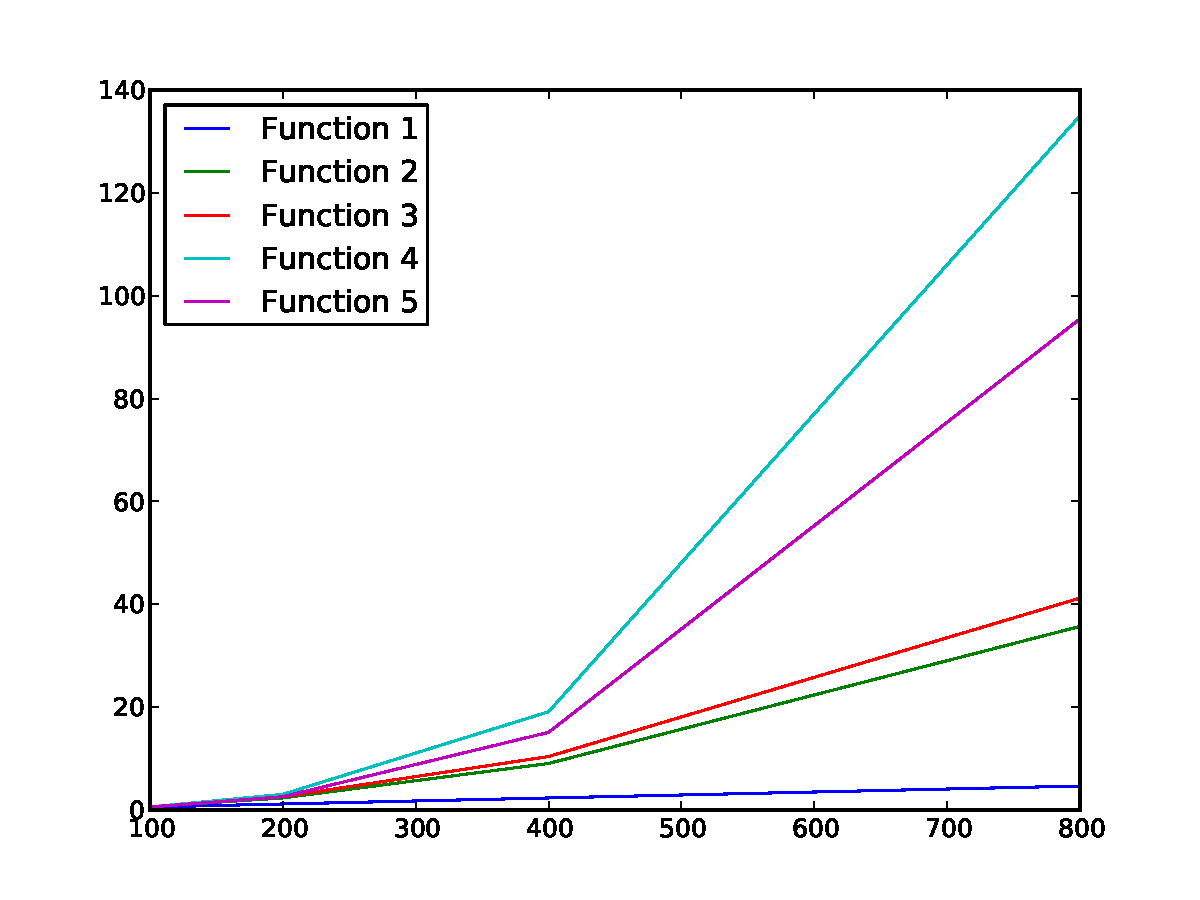
\includegraphics[width=\textwidth]{complexity_problem.pdf}

\end{problem}

\section*{Sparse Matrices}
A \emph{sparse} matrix is a matrix that has relatively few nonzero elements. 
Sparse matrices arise frequently in both theoretical and real-world applications. 
We can take advantage of the sparse structure of these matrices to use less memory and to decrease computation time.

For example, diagonal matrices are sparse. 
Storing an $n \times n$ diagonal matrix in the naive way means storing $n^2$ values in memory. 
For most applications, it makes more sense to store the diagonal entries in a 1-dimensional array of $n$ values. 
In addition to using less storage space, this allows for much faster matrix operations. 
Using the standard algorithm to multiply a matrix by a diagonal matrix involves $n^3$ steps, but most of these are multiplying by or adding zero. 
A smarter algorithm that knows all off-diagonal entries are zero can accomplish the same task much faster.

\subsection*{The Sparse Module}
The SciPy module \li{sparse} has storage methods to reduce the temporal and spatial complexity of handling sparse matrices.  
When we are not using these special methods, we say we are storing the \emph{full} matrix. 
We can also use \li{sparse} methods on dense matrices (matrices with mostly nonzero entries), but doing so will take longer than using the usual methods for handling full matrices. 

The difference in spatial complexity occurs because a full array occupies a block of memory for each entry, so an $n \times n$ array requires $n^2$ blocks of memory. 
By contrast, SciPy's \li{sparse} methods store only the nonzero entries and their locations in the array. 
As long as most entries are 0 (i.e., the matrix is sparse), this decreases spatial complexity. 
You minimize spatial complexity when you store a sparse matrix with the \li{sparse} module and a dense matrix as a full (or ``regular'') matrix.

SciPy has seven sparse matrix types, listed in Table \ref{table:smr}. 
Each type is optimized either for storing sparse matrices whose nonzero entries follow certain patterns, or for performing certain computations. 
For example, the \li{csc_matrix} and \li{csr_matrix} types are optimized for arithmetic operations. 
We will introduce some other types later in this lab. For more information, see the documentation (\url{http://docs.scipy.org/doc/scipy/reference/sparse.html}).




\begin{table}
\centering
\begin{tabular}{|r|l|}
\hline
Sparse Matrix Type & Description \\
\hline
\li{bsr_matrix} & Compressed Block Sparse Row\\
\li{coo_matrix} & Coordinate\\
\li{csc_matrix} & Compressed Sparse Column\\
\li{csr_matrix} & Compressed Sparse Row\\
\li{dia_matrix} & Sparse Diagonal\\
\li{dok_matrix} & Dictionary of Keys\\
\li{lil_matrix} & Linked List\\
\hline
\end{tabular}
\caption{Sparse matrix representations in SciPy.}
\label{table:smr}
\end{table}

Let us compare a \li{sparse} matrix computation with a full matrix computation. 
Note that we can convert any full matrix to a \li{sparse} matrix of any of the types listed in Table \ref{table:smr}.

\begin{lstlisting}
import numpy as np
from scipy import sparse

# Create a dense matrix (stored as a full matrix).
>>> A_full = np.random.rand(600, 600)

# Store A_full as a sparse matrix (even though it is dense).
>>> A_sparse = sparse.csc_matrix(A_full)

# Create a sparse matrix (stored as a full matrix).
>>> B_full = np.diag(np.random.rand(600))

# Store B_full as a sparse matrix.
>>> B_sparse = sparse.csc_matrix(B_full)

>>> def square(A):
        return np.power(A, 2)

>>> %timeit square(A_full)
100 loops, best of 3: 9.53 ms per loop

>>> %timeit square(A_sparse)
1 loops, best of 3: 941 ms per loop

>>> %timeit square(B_full)
100 loops, best of 3: 5.36 ms per loop

>>> %timeit square(B_sparse)
1000 loops, best of 3: 259 us per loop
\end{lstlisting}

As you can see from this example, we get the best performance when we store a sparse matrix with the \li{sparse} module and a dense matrix as a full matrix.

\begin{comment}
\begin{problem}
Create a $500\times 500$ matrix and vector of length 500, both full of random values. Use the \li{A.dot(b)} command to multiply your matrix and your vector, and time how long it takes to do so. Then convert your matrix to sparse format and again time how long it takes to multiply it by your vector using \li{A.dot(b)}.
\end{problem}
\end{comment}

\subsection*{Creating Sparse Matrices}
One way to create a sparse matrix is to create a full matrix and then convert it to a sparse matrix, as we did in the previous example. 
However, you reduce spatial complexity if you never create the full matrix. 
Here are two ways to create sparse matrices directly.

The first way is to use the method \li{sparse.spdiags(data, diags, m, n)}. 
If \li{data} is a 1-D array and \li{diags} is a scalar, then this method creates an $m \times n$ matrix with \li{data} on the specified diagonal. 
The parameter \li{diags=0} indicates the main diagonal, with lower diagonals indexed by negative numbers and upper diagonals by positive numbers. 
If \li{data} is a 2-D array and \li{diags} is a list, then this method creates an $m \times n$ matrix with the rows of \li{data} on the diagonals specified by \li{diags}. 
See the documentation for more information.
\begin{lstlisting}
# Create a sparse 3x3 matrix with (2, 3, 4) on the diagonal.
>>> A = sparse.spdiags([2, 3, 4], 0, 3, 3)
>>> A
<3x3 sparse matrix of type '<type 'numpy.int64'>'
	with 3 stored elements (1 diagonals) in DIAgonal format>
# Convert A to a full matrix.
>>> A.todense()
matrix([[2, 0, 0],
        [0, 3, 0],
        [0, 0, 4]])
	
# Create a sparse 4x4 matrix with the rows of diag_entries on the diagonals.
>>> diag_entries = np.array([[3,6,9,0],[1,4,7,10],[0,2,5,8]])
>>> B = sparse.spdiags(diag_entries, [-1, 0, 1], 4, 4)
<4x4 sparse matrix of type '<type 'numpy.int64'>'
	with 10 stored elements (3 diagonals) in DIAgonal format>
>>> B.todense()
matrix([[ 1,  2,  0,  0],
        [ 3,  4,  5,  0],
        [ 0,  6,  7,  8],
        [ 0,  0,  9, 10]])
\end{lstlisting}

The final matrix $B$ in the example above is a special kind of matrix called a \emph{banded} matrix. 
A banded matrix is a sparse matrix whose only non-zero entries are on the main diagonal and some diagonals on either side. 
In fact, $B$ is an example of a \emph{tri-diagonal} matrix, because its nonzero entries are confined to the three central diagonals. 
Banded matrices arise naturally in many applications, including numerical methods for solving differential equations. 

\begin{problem}
Write a function that takes an integer argument \li{n} and returns a sparse $n\times n$
tri-diagonal array with $2$'s along the diagonal and $-1$'s along
the two sub-diagonals above and below the diagonal. 
The array should be in \li{csr_matrix} format.
\emph{Hint}: Read about the \li{format} keyword parameter of the \li{sparse.spdiags} method.

This matrix is the derivative operator in numerical analysis of differential equations.
\label{prob:sparse_tridiag}
\end{problem}

A second way to create a sparse matrix is to pre-allocate an array of zeros and then specify the nonzero entries one at a time. 
The most efficient sparse matrix types for building matrices incrementally are \li{lil_matrix} and \li{dok_matrix}. 
Once you are done constructing the sparse matrix, you should convert it to a form that is optimized for computations.


\begin{lstlisting}
# Initialize Z.
>>> Z = sparse.lil_matrix((400, 300))
# Specify the nonzero entries of Z.
>>> Z[1,34] = 23
>>> Z[23,32] = 56
>>> Z[2,:] = 13.2
>>> Z
<400x300 sparse matrix of type '<type 'numpy.float64'>'
	with 302 stored elements in LInked List format>

\end{lstlisting}

When the matrix \li{Z} is initialized, all its entries are assumed to be zero. 
Note that at the end of \li{Z}'s construction, only 302 elements are being stored for a matrix with 120000 entries. 

You may have noticed that the only way to view a matrix as a 2-D array is to convert it to a full matrix. 
If your matrix is too large to do this, you can still visualize it using the \li{plt.spy()} command from matplotlib. 
This function plots the locations of the non-zero entries in a matrix. 
The following code outputs Figure \ref{fig:mpl_spy}.

\begin{lstlisting}
>>> from matplotlib import pyplot as plt
>>> B = np.random.rand(3, 10000)
>>> A = sparse.spdiags(B, range(-1, 2), 10000, 10000)
>>> plt.spy(A)
\end{lstlisting}

\begin{figure}
\centering
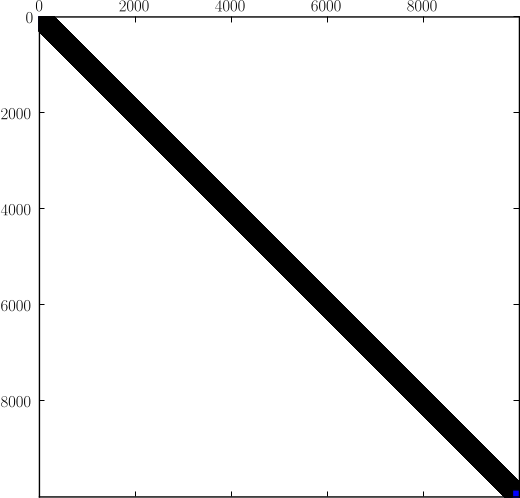
\includegraphics[width=.75\textwidth]{spy.png}
\caption{The output of the \li{spy()} command}
\label{fig:mpl_spy}
\end{figure}


%insert problem here that lets them play around with large sparse matrices in diff forms


\begin{comment}
\subsection*{Banded Matrices}
\begin{problem}
Write a function that takes an integer argument \li{n} and returns a full $n\times n$
tri-diagonal array with $2$'s along the diagonal and $-1$'s along
the two sub-diagonals above and below the diagonal.
\emph{Helpful Hint}: Use the \li{np.diagflat()} command.
\label{full_tridiag}
\end{problem}
\end{comment}

\subsection*{Manipulating Sparse Matrices}
Scipy's \li{sparse} matrices behave a little differently than NumPy arrays.
You can multiply two sparse matrices element-wise with the \li{multiply()} method of one of the sparse matrices.
\begin{lstlisting}
>>> D = sparse.spdiags([2,3,4],0,3,3)
>>> C = sparse.spdiags(np.ones((3,3)), [-1,0,1], 3, 3)
>>> (D.multiply(C)).todense()
matrix([[ 2.,  0.,  0.],
        [ 0.,  3.,  0.],
        [ 0.,  0.,  4.]])
\end{lstlisting}

On the other hand, the asterisk \li{*} performs ordinary matrix multiplication. 
You can also use the \li{dot} method of one of the sparse matrices. 
However, you should NOT use \li{np.dot} on sparse matrices because it may return an incorrect answer.
\begin{lstlisting}
# One correct way to mutliply sparse matrices
>>> (D.dot(C)).todense()
matrix([[ 2.,  2.,  0.],
        [ 3.,  3.,  3.],
        [ 0.,  4.,  4.]])
\end{lstlisting}

Addition and scalar multiplication are implemented as usual.
\begin{lstlisting}
>>> (D + 3*C).todense()
matrix([[ 5.,  3.,  0.],
        [ 3.,  6.,  3.],
        [ 0.,  3.,  7.]])
\end{lstlisting}




\section*{Using Sparse Matrices to Reduce Runtimes}
In addition to spatial complexity, the \li{sparse} module can reduce temporal complexity. 
Consider the linear system $A x = b$, where $A$ is a $100000\times 100000$ tri-diagonal matrix.
Storing a full matrix of that size requires 10 billion double-precision floating-point numbers. 
Since it takes 8 bytes to store a double, we need roughly 80GB to store the full matrix. 
Lack of storage space makes this system impossible to solve for most desktop computers, but even more problematic is the temporal complexity. 
Methods for directly solving a linear system are usually $O(n^3)$. 
As a result, even if the computer could store an 80GB matrix in RAM, it would still take several weeks to solve the system. 
%However, since we don't typically have computers with that much available RAM, most of the
%matrix would have to be stored on the hard drive, so the computation would probably take between $6$ months to a year.

The point is, even as computers increase in processing speed and memory, we can still easily construct problems that they will struggle to solve in a reasonable amount of time. 
However, if we store the tri-diagonal matrix as a \li{sparse} matrix, we can solve the linear system, even with a modest computer. 

Let's first compute the spatial complexity of the above system when $A$ is stored as a sparse matrix. 
There are three diagonals that have roughly $100000$ non-zero entries. 
That's $300000$ double-precision floating point numbers, which is about 2.4 MB, or less storage than your favorite song. 
Thus, the sparse matrix will easily fit into the computer's RAM. Furthermore, the temporal complexity for solving a tri-diagonal matrix is $O(n)$.
\footnote{Because there are fast algorithms for solving a tri-diagonal linear system, you may think that there are fast algorithms for inverting a tri-diagonal matrix. 
In fact this is not true, and the inverse of a sparse matrix is usually not sparse. 
There is rarely a good reason to invert a matrix, sparse or dense.} 
Let's see how long it takes to solve the system when $A$ and $b$ are filled with random data.

\begin{lstlisting}
>>> from scipy.sparse import linalg as sl
>>> G = np.random.rand(3, 100000)
>>> b = np.random.rand(1, 100000)
>>> A = sparse.spdiags(G,[-1,0,1],100000,100000, format='csr')
>>> def solSys():
...     return sl.spsolve(A, b)

>>> %timeit solSys()
1 loops, best of 3: 80.8 ms per loop

\end{lstlisting}

This computer solved the system in only 80.8 milliseconds.

\begin{comment}
\begin{problem}
Write a function that accepts an integer argument \li{n} as well as a keyword argument \li{sparse} whose value is either \li{True} or \li{False} (default to \li{False}). 
Then do the following:
\begin{enumerate}
\item Inside of the function, use your previous solutions to generate an $n \times n$ tri-diagonal array $A$ -- either sparse or full depending on the value of the \li{sparse} argument.
\item Generate an $n \times 1$ random array $b$
\item Solve the system $Ax = b$, using either \li{scipy.sparse.linalg.spsolve} or \li{scipy.linalg.solve}
(again depending on the value of \li{sparse}) and return the solution.
\item Time the function for \li{n = 2000} using both the sparse and the full option.
\end{enumerate}
\end{problem}
\end{comment}


\begin{problem}
Write a function that accepts an integer argument $n$ and does the following:
\begin{enumerate}
\item Generates an $n \times 1$ random array $b$.
\item Solves the linear system $Ax = b$, where $A$ is the tri-diagonal array in Problem \ref{prob:sparse_tridiag} of size $n \times n$.
\end{enumerate}
\end{problem}



\begin{problem}
Write a function that accepts an integer argument \li{n} and returns $\lambda n^2$, where
$\lambda$ is the smallest eigenvalue of the sparse tri-diagonal array you built in Problem \ref{prob:sparse_tridiag}.

If \li{A} is your tri-diagonal matrix, calculate $\lambda$ using the method \li{scipy.sparse.linalg.eigs} with the command \li{sl.eigs(A.asfptype(), which = 'SM')}. 
The code \li{A.asfptype()} ensures that your matrix has the right data type, and the parameter \li{which = 'SM'} tells the function to look for the smallest eigenvalues. 
This command will return several of the smallest eigenvalues of \li{A}, and you will have to select the smallest of these. 
Read the documentation of \li{sl.eigs} for more information.

What value does $\lambda n^2$ approach as $n$ approaches infinity? 
This value is meaningful in operator theory. 
\li{Hint}: This value is the square of an important number.

\end{problem}





 
